\section{Prove effettuate}
\label{prove}
%Qui inseriremo le prove effettuate con il nostra progetto, insieme all'elenco dei beacon utilizzati, alla loro disposizione, al loro scopo e ai loro dati. Sar� infine aggiunta una valutazione dell'esito della prova.
Durante la realizzazione di questo progetto sono stati effettuati alcuni test per verificare che tutto il sistema funzionasse correttamente. In questa sezione essi verranno descritti, in particolare per quanto riguarda la disposizione e le impostazioni dei beacon, insieme all'esito finale e ai problemi da risolvere sorti durante la loro esecuzione.
	\subsection{Percorso di prova ufficiale della Revisione di Accettazione}
		Non � un test ma un percorso ufficiale vero e proprio, � stato aggiunto in questa sezione perch� l'esito ottenuto ha portato a individuare dei miglioramenti da implementare per il percorso finale.
		Il percorso consiste in 3 stazioni da giocare nell'edificio Torre Archimede dell'Universit� degli Studi di Padova. La partenza, ovvero quando viene premuto il pulsante di inizio percorso, � al primo piano nell'aula 1C150, mentre la prima tappa � situata vicino all'entrata della biblioteca, al primo piano interrato. All'inizio quindi � stato verificato che i beacon della altre tappe vengono scartati quando sono rilevati. Giocata la prima tappa il percorso prevede che l'utente torni per la stessa strada della partenza, stavolta per� pu� giocare le altre tappe, visto che vengono rilevati in ordine i beacon della seconda e della terza tappa.
	
		\begin{tabella}{!{\VRule}l!{\VRule}l!{\VRule}l!{\VRule}} %TODO: aggiungere dati dispositivo usato
			\intestazionethreecol{Nome dispositivo}{Versione Android}{Note sull'esito della prova}
			 && && \\
			\caption{Tabella con i dati dei dispositivi usati per il percorso}
		\end{tabella}
	
		\subsubsection{Dati e disposizione dei beacon}
	
		\begin{figure}[!h]
				\centering
				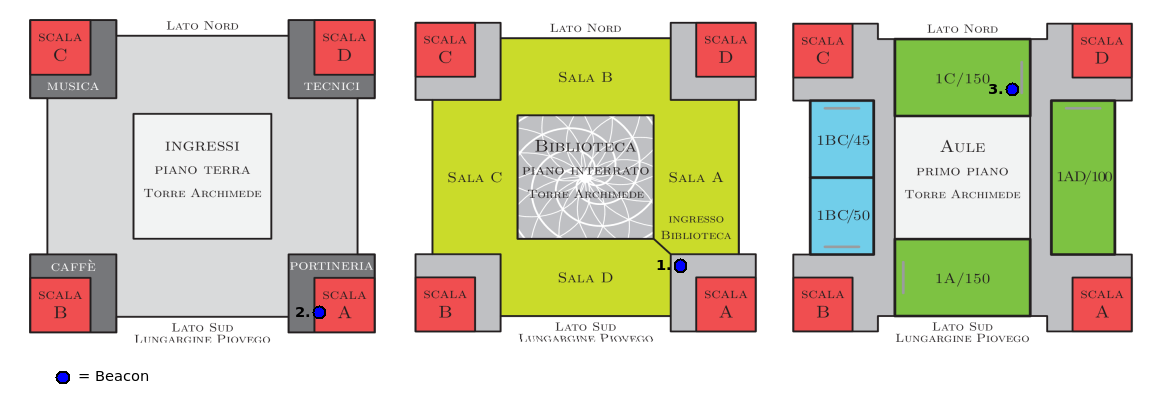
\includegraphics[scale=0.5]{planimetrie/TorreArchimede}  
				\caption{Planimetria della Torre Archimede con la posizione dei beacon segnata}
		\end{figure}
	
		\begin{tabella}{!{\VRule}l!{\VRule}l!{\VRule}l!{\VRule}l!{\VRule}l!{\VRule}l!{\VRule}}
			\intestazionesixcol{Numero beacon}{UUID}{Major}{Minor}{Potenza (dBm)}{Note posizione}
			1. && f7826da6-4fa2-4e98-8024-bc5b71e0893e && 0 && 0 && -20 && \\
			2. && f7826da6-4fa2-4e98-8024-bc5b71e0893e && 1 && 0 && -12 && Beacon posizionato davanti a una finestra della scala. � richiesta pi� potenza per coprire tutta l'area \\
			3. && f7826da6-4fa2-4e98-8024-bc5b71e0893e && 2 && 0 && -20 && \\
			\caption{Tabella con i dati dei beacon usati per il percorso}
		\end{tabella}
	
		\subsubsection{Esito della prova}
		La prova ha avuto successo, all'andata sono stati esclusi i beacon delle altre tappe e al ritorno sono stati rilevati in un tempo accettabile, inoltre le funzioni mostrate sono state eseguite come previsto.
		A seguito di questa prova e dei test eseguiti in precedenza per la sua preparazione abbiamo individuato delle modifiche abbastanza importanti da apportare, come l'aggiunta delle proximity, ovvero le interfacce che, quando rilevano un determinato beacon, comunicano all'utente quanto manca per raggiungere la prossima stazione, oppure un miglioramento della gestione degli errori che possono essere restituiti dal server.
	\subsection{Test sul funzionamento delle Proximity}
		In questo test � stato verificato che le classi relative al funzionamento delle Proximity funzionassero correttamente. Per eseguire il test abbiamo preso quattro beacon, due per le prime due prove del percorso e due per due proximity presenti tra la prima e la seconda prova. Il percorso usato � quello preparato per la Revisione di Accettazione, ma sono stati usati solo una parte dei beacon necessari, quindi esso non � stato portato a termine.
	
		\begin{tabella}{!{\VRule}l!{\VRule}l!{\VRule}l!{\VRule}}
			\intestazionethreecol{Nome dispositivo}{Versione Android}{Note sull'esito della prova}
			 && && \\
			\caption{Tabella con i dati dei dispositivi usati per il percorso}
		\end{tabella}
	
		\subsubsection{Dati e disposizione dei beacon}
		I beacon sono stati disposti lungo un corridoio dritto in Torre Archimede, quindi seguendo una linea retta. Pi� precisamente sono stati posati sul davanzale interno all'edificio, quindi a circa 110 cm di altezza.
	
		\begin{tabella}{!{\VRule}l!{\VRule}l!{\VRule}l!{\VRule}l!{\VRule}l!{\VRule}l!{\VRule}}
			\intestazionesixcol{Numero beacon}{UUID}{Major}{Minor}{Potenza (dBm)}{Note posizione}
			1. && f7826da6-4fa2-4e98-8024-bc5b71e0893e && 0 && 0 && -30 && \\
			2. && f7826da6-4fa2-4e98-8024-bc5b71e0893e && 5 && 0 && -30 && \\
			3. && f7826da6-4fa2-4e98-8024-bc5b71e0893e && 4 && 0 && -30 && \\
			4. && f7826da6-4fa2-4e98-8024-bc5b71e0893e && 1 && 0 && -30 && \\
			\caption{Tabella con i dati dei beacon usati per il percorso}
		\end{tabella}
	
		\subsubsection{Esito della prova}
		La prova ha avuto successo, anche se sono stati rilevati degli errori nelle classi da verificare, prontamente risolti al momento. La cosa forse pi� preoccupante � la difficolt� nel gestire il raggio massimo in cui il beacon pu� essere rilevato, anche se probabilmente era dovuto all'errore nelle classi delle Proximity. Si vedr� durante la prova del percorso per Miriade se riscontreremo ancora problemi di questo tipo.
	\subsection{Test generale del percorso per Miriade}
		In questo test � stato verificato che il percorso da presentare a Miriade il 30 settembre funzionasse correttamente, oltre a impostare la potenza dei beacon pi� adatta alla loro posizione.
	
		\begin{tabella}{!{\VRule}l!{\VRule}l!{\VRule}l!{\VRule}}
			\intestazionethreecol{Nome dispositivo}{Versione Android}{Note sull'esito della prova}
			 && && \\
			\caption{Tabella con i dati dei dispositivi usati per il percorso}
		\end{tabella}
	
		\subsubsection{Dati e disposizione dei beacon}
		I primi 8 beacon sono quelli delle stazioni, i rimanenti invece sono usati dalle proximity.
	
		\begin{tabella}{!{\VRule}l!{\VRule}l!{\VRule}l!{\VRule}l!{\VRule}l!{\VRule}l!{\VRule}}
			\intestazionesixcol{Numero beacon}{UUID}{Major}{Minor}{Potenza (dBm)}{Note posizione}
			1. && f7826da6-4fa2-4e98-8024-bc5b71e0893e && 0 && 0 && -30 && \\
			2. && f7826da6-4fa2-4e98-8024-bc5b71e0893e && 0 && 1 && -30 && \\
			3. && f7826da6-4fa2-4e98-8024-bc5b71e0893e && 0 && 2 && -30 && � il beacon sia della terza stazione sia dell'ottava \\
			4. && f7826da6-4fa2-4e98-8024-bc5b71e0893e && 0 && 3 && -30 && \\
			5. && f7826da6-4fa2-4e98-8024-bc5b71e0893e && 0 && 4 && -30 && \\
			6. && f7826da6-4fa2-4e98-8024-bc5b71e0893e && 0 && 5 && -30 && \\
			7. && f7826da6-4fa2-4e98-8024-bc5b71e0893e && 0 && 6 && -30 && \\
			8. && f7826da6-4fa2-4e98-8024-bc5b71e0893e && 0 && 7 && -30 && \\
			9. && f7826da6-4fa2-4e98-8024-bc5b71e0893e && 0 && 9 && -30 && \\
			10. && f7826da6-4fa2-4e98-8024-bc5b71e0893e && 0 && 10 && -30 && \\
			11. && f7826da6-4fa2-4e98-8024-bc5b71e0893e && 0 && 11 && -30 && \\
			12. && f7826da6-4fa2-4e98-8024-bc5b71e0893e && 0 && 12 && -30 && \\
			13. && f7826da6-4fa2-4e98-8024-bc5b71e0893e && 0 && 13 && -30 && \\
			14. && f7826da6-4fa2-4e98-8024-bc5b71e0893e && 0 && 14 && -30 && \\
			\caption{Tabella con i dati dei beacon usati per il percorso}
		\end{tabella}
	
		\subsubsection{Esito della prova}
		La prova ha avuto successo, anche se la distanza a cui il beacon viene rilevato cambia in modo significativo a seconda del dispositivo. Questo potrebbe causare problemi dentro a luoghi abbastanza piccoli, perch� porterebbe a rilevare dei beacon che in teoria dovrebbero essere distanti. Nel complesso comunque non dovrebbero esserci risultati che compromettano l'esecuzione del percorso.